\documentclass[aspectratio=169,10pt]{beamer}

\usepackage[T1]{fontenc}
\usepackage{lmodern}
\usepackage{amsmath,amssymb}
\usepackage{graphicx}
\usepackage{booktabs,tabularx,array}
\usepackage{tikz}
\usepackage{pgfplots}
\pgfplotsset{compat=1.18}
\usetikzlibrary{arrows.meta,positioning,calc}

\definecolor{Ink}{HTML}{17313A}
\definecolor{Teal}{HTML}{087F72}
\definecolor{Green}{HTML}{178C4A}
\definecolor{Blue}{HTML}{3F78B8}
\definecolor{Orange}{HTML}{D97722}
\definecolor{Red}{HTML}{C83D3D}
\definecolor{Paper}{HTML}{FBFCFA}
\definecolor{Muted}{HTML}{5C7076}

\setbeamercolor{normal text}{fg=Ink,bg=Paper}
\setbeamercolor{structure}{fg=Teal}
\setbeamercolor{frametitle}{fg=Ink,bg=Paper}
\setbeamerfont{frametitle}{size=\Large,series=\bfseries}
\setbeamertemplate{navigation symbols}{}
\setbeamertemplate{footline}{%
  \hfill\color{Muted}\scriptsize\insertframenumber\, /\, 10\hspace{0.45cm}\vspace{0.22cm}}
\setbeamertemplate{itemize item}{\color{Teal}\small$\blacktriangleright$}
\setbeamertemplate{itemize subitem}{\color{Green}\scriptsize$\bullet$}

\title{An ML-Driven Energy Auditing and Automated Decision System for Turkish Textile SMEs}
\author{Furkan Kalkan & Liang Chengxin}
\date{2026}

\begin{document}

% 1 — Project framing
\begin{frame}[plain]
  \vspace*{0.08cm}
  {\color{Teal}\small COURSE PROJECT \hfill TURKISH TEXTILE SMEs}\par
  \vspace{0.18cm}
  {\bfseries\fontsize{22}{26}\selectfont\color{Ink}
  An ML-Driven Energy Auditing and Automated
  Decision System for Turkish Textile SMEs}\par
  \vspace{0.25cm}
  {\color{Teal}\rule{1.25cm}{2.2pt}}\par
  \vspace{0.20cm}
  \textbf{Application area:} Industrial energy auditing and automated decision support for textile SMEs.\par
  \vspace{0.13cm}
  \textbf{Project goal:} Help Turkish textile small and medium enterprises (SMEs) reduce electricity cost and carbon emissions, extend machine life, and preserve production throughput.\par
  \vspace{0.13cm}
  \textbf{Target customer:} A spinning, weaving and dyeing SME with ring-spinning motors, compressed air, dyeing circulation pumps, and humidity/HVAC loads.
\end{frame}

% 2 — Sensor model and anomaly detection
\begin{frame}{From machine signals to an explainable warning}
\normalsize
\textbf{1. Measure each asset every 15 minutes}\par
\vspace{1mm}
Power $P_{m,t}$, temperature $T_{m,t}$, vibration $V_{m,t}$, and production $q_{m,t}$. For $\Delta t=0.25$ hour:
\[
  E_{m,t}=P_{m,t}\Delta t,\qquad
  EnergyPerUnit_{m,t}=\frac{E_{m,t}}{\max(q_{m,t},\epsilon)}.
\]
\vspace{-2mm}
\textbf{2. Compare readings with each machine's baseline}\par
\[
  \Delta T_{m,t}=T_{m,t}-T_m^{base},\qquad
  \Delta V_{m,t}=V_{m,t}-V_m^{base}.
\]
\vspace{-2mm}
\textbf{3. Find unusual combinations, not just one high sensor value}\par
\[
  z_{m,t}=[EnergyPerUnit,\Delta T,\Delta V,\text{load ratio},\ldots],\qquad
  A_{m,t}=\mathbf{1}\{s(z_{m,t})<\tau\}.
\]
\normalsize
Here, $s(\cdot)$ is the Isolation Forest score and $\tau$ is its alert threshold. The forest finds unusual patterns; physical rules and operating context help explain them.
\end{frame}

% 3 — Optimization story
\begin{frame}{A production schedule with cost, carbon and health in view}
\small
For machine $m$ and hour $h$, choose production $x_{m,h}$, run/batch status $y_{m,h}\in\{0,1\}$, power $p_{m,h}$, and factory peak $D$.
\[
\min J=\lambda_C\frac{C}{C_0}+\lambda_D\frac{D}{D_0}
       +\lambda_G\frac{G}{G_0}+\lambda_H\frac{R}{R_0}
\]
\vspace{-2mm}
\[
C=\sum_{m,h}c_h p_{m,h}\Delta t,\quad
G=\sum_{m,h}g_h p_{m,h}\Delta t,\quad
D\geq\sum_m p_{m,h}\;\;\forall h.
\]
\vspace{-2mm}
\begin{columns}[T,onlytextwidth]
\column{0.53\textwidth}
\textbf{Keep production on target}
\[
\sum_h x_{m,h}=Q_m,\qquad
q_m^{min}y_{m,h}\leq x_{m,h}\leq q_m^{max}y_{m,h}.
\]
\column{0.44\textwidth}
\textbf{Respect the machine and process}
\[
p_{m,h}=P_m^{idle}y_{m,h}+\alpha_m x_{m,h},\quad
p_{m,h}\leq P_m^{max}a_{m,h}.
\]
\end{columns}
\vspace{-2mm}
\footnotesize
$C$: electricity bill; $D$: coincident peak; $G$: Carbon emissions; $R$: condition-risk proxy. Weights $\lambda$ set factory priorities. Availability $a_{m,h}$ reflects maintenance and health limits. Add HVAC-to-spinning support and three-hour dyeing batches. Rates $c_h$ use the Turkish scenario tariff.
\end{frame}

% 4 — Success criteria
\begin{frame}{criteria}
\normalsize
\begin{columns}[T,onlytextwidth]
\column{0.49\textwidth}
{\color{Teal}\bfseries FACTORY / BUSINESS}\par\vspace{2mm}
\begin{itemize}\setlength\itemsep{2pt}
  \item Electricity cost: TRY/day and change from baseline
  \item Energy use: kWh/day and kWh per kg of yarn
  \item Carbon emission: kg CO$_2$e/day and kg CO$_2$e/kg yarn
  \item Production: output target met; no lost throughput
  \item Peak demand: highest coincident kW
  \item Machine condition: ISO 10816-3 vibration zone
\end{itemize}
\column{0.49\textwidth}
{\color{Blue}\bfseries AI / MODEL}\par\vspace{2mm}
\begin{itemize}\setlength\itemsep{2pt}
  \item Precision: how many alerts were real faults?
  \item Recall: how many labeled faults were found?
  \item F1 score: balance between precision and recall
  \item False alarms during normal operation
  \item Results are measured on labeled synthetic records
\end{itemize}
\end{columns}
\vspace{1mm}
\footnotesize\textbf{ISO vibration guide (machine class II):} A $\leq 2.3$; B 2.3--4.5; C 4.5--7.1; D $>7.1$ mm/s RMS. Zone C needs action; Zone D is unacceptable.
\end{frame}

% 5 — Pipeline
\begin{frame}{Workflow: from sensors to a plant action}
\normalsize
\begin{enumerate}\setlength\itemsep{3pt}
  \item[\textcolor{Teal}{\bfseries 1}] \textbf{Sensors} --- Meters and CTs measure power; temperature, vibration, and production readings add machine context.
  \item[\textcolor{Teal}{\bfseries 2}] \textbf{Industrial features and data checks} --- Calculate energy per unit, EnergyPerUnit, thermal elevation, and load. Flag missing, duplicate, or out-of-range readings; clean data transparently.
  \item[\textcolor{Teal}{\bfseries 3}] \textbf{Multivariate Isolation Forest} --- Find unusual sensor combinations and assign Normal, Medium, High, or Critical severity.
  \item[\textcolor{Teal}{\bfseries 4}] \textbf{Explainable condition engine} --- Add operating context and ISO 10816-3 zones; report evidence $\rightarrow$ model inference $\rightarrow$ likely cause $\rightarrow$ recommended check.
  \item[\textcolor{Teal}{\bfseries 5}] \textbf{PuLP mixed-integer schedule} --- Set machine on/off and output levels within health, tariff, batch, and production limits; compare cost, peak demand, and carbon impact.
\end{enumerate}
\end{frame}

% 6 — 24-hour tariff and peak demand chart, updated with the Turkey scenario output
\begin{frame}{Time-of-use load shifting and coincident peak demand}
\begin{center}
\small\color{Muted}Turkey scenario rates: peak 5.50 TRY/kWh \quad day 4.50 TRY/kWh \quad night 3.50 TRY/kWh
\end{center}
\vspace{-2mm}
\begin{center}
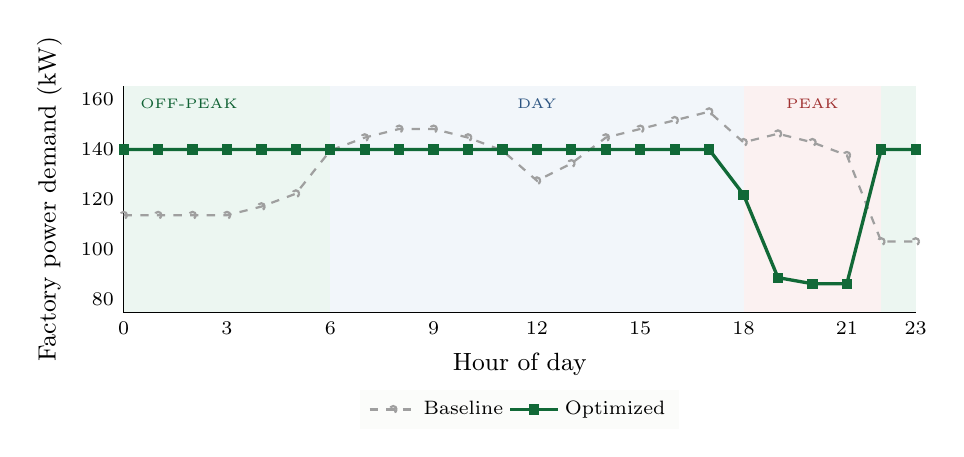
\begin{tikzpicture}
\begin{axis}[
  width=0.96\linewidth,height=4.45cm,
  xmin=0,xmax=23,ymin=75,ymax=165,
  xlabel={Hour of day},ylabel={Factory power demand (kW)},
  xtick={0,3,6,9,12,15,18,21,23},
  tick label style={font=\scriptsize},label style={font=\small},
  grid=major,grid style={draw=Ink!12},
  legend style={font=\scriptsize,draw=none,fill=Paper,at={(0.5,-0.34)},anchor=north,legend columns=2},
  clip=false
]
\path[fill=Green!8] (axis cs:0,75) rectangle (axis cs:6,165);
\path[fill=Blue!7] (axis cs:6,75) rectangle (axis cs:18,165);
\path[fill=Red!7] (axis cs:18,75) rectangle (axis cs:22,165);
\path[fill=Green!8] (axis cs:22,75) rectangle (axis cs:23,165);
\node[font=\tiny,text=Green!70!black,anchor=north west] at (axis cs:0.2,164) {OFF-PEAK};
\node[font=\tiny,text=Blue!70!black,anchor=north] at (axis cs:12,164) {DAY};
\node[font=\tiny,text=Red!80!black,anchor=north] at (axis cs:20,164) {PEAK};
\addplot[gray!75,thick,dashed,mark=o,mark size=1.2pt] coordinates {
  (0,113.64)(1,113.64)(2,113.64)(3,113.64)(4,117.08)(5,122.22)(6,139.42)(7,144.57)
  (8,148.01)(9,148.01)(10,144.57)(11,139.42)(12,127.39)(13,134.26)(14,144.57)(15,148.01)
  (16,151.45)(17,154.89)(18,142.68)(19,146.12)(20,142.68)(21,137.52)(22,103.14)(23,103.14)};

\addlegendentry{Baseline}
\addplot[Green!75!black,very thick,mark=square*,mark size=1.25pt] coordinates {
  (0,139.86)(1,139.85)(2,139.85)(3,139.85)(4,139.85)(5,139.85)(6,139.85)(7,139.85)
  (8,139.85)(9,139.85)(10,139.85)(11,139.85)(12,139.85)(13,139.85)(14,139.85)(15,139.85)
  (16,139.85)(17,139.85)(18,121.85)(19,88.77)(20,86.34)(21,86.34)(22,139.85)(23,139.85)};
\addlegendentry{Optimized}
\end{axis}
\end{tikzpicture}
\end{center}
\vspace{-3mm}
\begin{center}\normalsize
Peak: 154.89 $\rightarrow$ 139.86 kW (\textbf{15.03 kW / 9.70\% lower})\quad
Daily cost: TRY 14,040.96 $\rightarrow$ TRY 13,575.85 (\textbf{TRY 465.11 / 3.31\% saved})
\end{center}
\vspace{-1mm}
\scriptsize\color{Muted}Hourly profiles are from the current synthetic Turkey scenario. Flexible dyeing batches move away from the 18:00--22:00 peak; off-peak load can rise as a result.
\end{frame}

% 7 — Recreated benchmark chart from source slide 8 metrics
\begin{frame}{Condition monitoring: physics plus AI reduces false alarms}
\begin{columns}[T,onlytextwidth]
\column{0.64\textwidth}
\centering
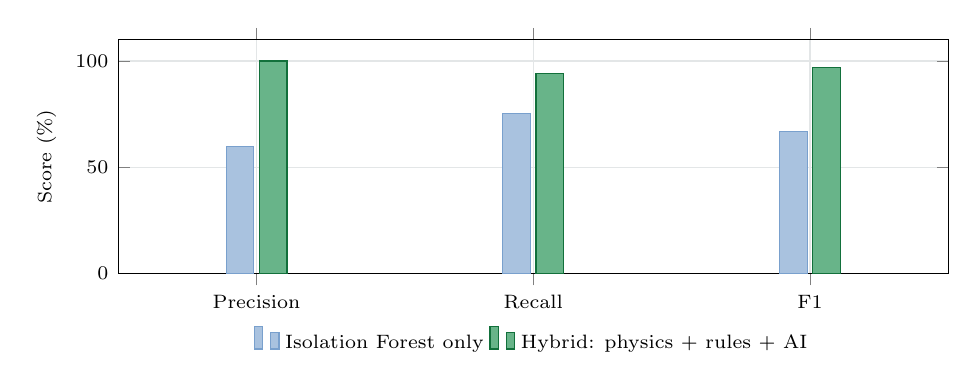
\begin{tikzpicture}
\begin{axis}[
  ybar,bar width=10pt,width=\linewidth,height=4.55cm,
  symbolic x coords={Precision,Recall,F1},xtick=data,
  ymin=0,ymax=110,ylabel={Score (\%)},
  tick label style={font=\scriptsize},label style={font=\scriptsize},
  grid=major,grid style={draw=Ink!12},
  legend style={font=\scriptsize,draw=none,at={(0.5,-0.20)},anchor=north,legend columns=2},
  enlarge x limits=0.25
]
\addplot[fill=Blue!45,draw=Blue!70] coordinates {(Precision,59.85)(Recall,75.24)(F1,66.67)};
\addlegendentry{Isolation Forest only}
\addplot[fill=Green!65,draw=Green!80!black] coordinates {(Precision,100)(Recall,94.29)(F1,97.06)};
\addlegendentry{Hybrid: physics + rules + AI}
\end{axis}
\end{tikzpicture}
\column{0.34\textwidth}
\centering
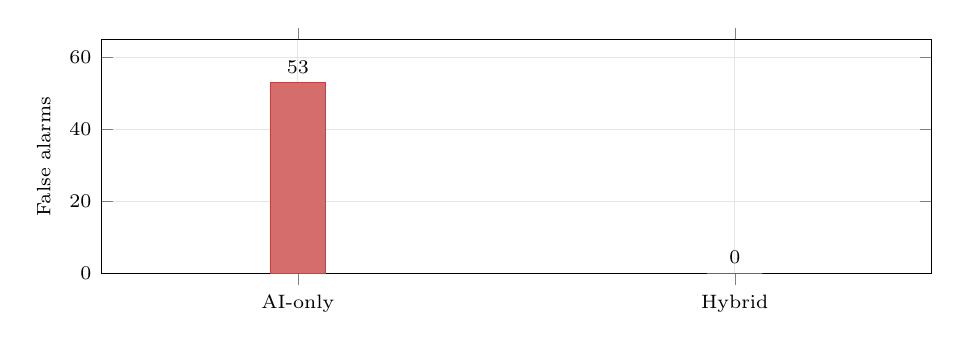
\begin{tikzpicture}
\begin{axis}[
  ybar,bar width=20pt,width=\linewidth,height=4.55cm,
  symbolic x coords={AI-only,Hybrid},xtick=data,
  xticklabel style={font=\scriptsize},
  ymin=0,ymax=65,ylabel={False alarms},
  ytick={0,20,40,60},tick label style={font=\scriptsize},label style={font=\scriptsize},
  nodes near coords,every node near coord/.append style={font=\scriptsize},
  grid=major,grid style={draw=Ink!12},enlarge x limits=0.45
]
\addplot[fill=Red!75,draw=Red] coordinates {(AI-only,53)(Hybrid,0)};
\end{axis}
\end{tikzpicture}
\end{columns}
\vspace{1mm}
\centering\small Hybrid: \textbf{100\% precision}, \textbf{94.29\% recall}, \textbf{97.06\% F1}.\\
\scriptsize\color{Muted}5,248 labeled synthetic operational samples; not a field trial. ISO and operating context suppress normal idle-break alerts.
\end{frame}

% 8 — Carbon calculation, refreshed to the Turkey factor and current run
\begin{frame}{Less wasted energy means lower Carbon emissions}
\vspace{2mm}
\begin{center}
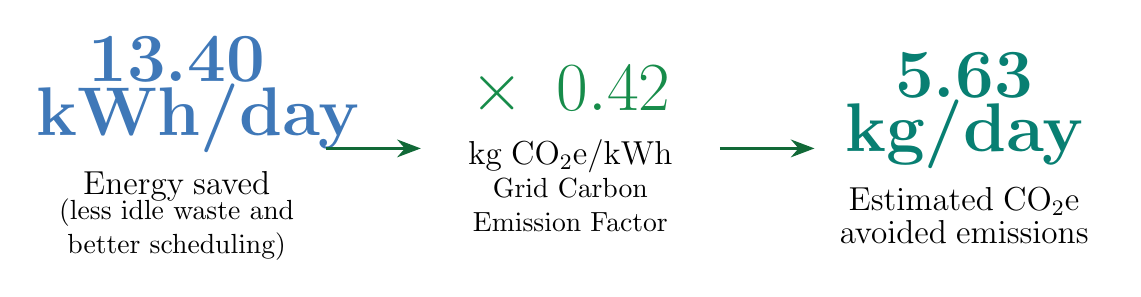
\begin{tikzpicture}[
  flowbox/.style={align=center,text width=3.55cm,minimum height=2.2cm},
  link/.style={-{Stealth[length=3mm]},line width=1.1pt,draw=Green!75!black}
]
\node[flowbox] (energy) at (0,0) {{\color{Blue}\bfseries\fontsize{23}{26}\selectfont 13.40 kWh/day}\\[2mm]
  \large Energy saved\\[-1mm]\normalsize(less idle waste and better scheduling)};
\node[flowbox] (factor) at (5.0,0) {{\color{Green}\bfseries\fontsize{23}{26}\selectfont $\times\;0.42$}\\[2mm]
  \large kg CO$_2$e/kWh\\{\normalsize Grid Carbon Emission Factor}};
\node[flowbox] (daily) at (10.0,0) {{\color{Teal}\bfseries\fontsize{23}{26}\selectfont 5.63 kg/day}\\[2mm]
  \large Estimated CO$_2$e avoided emissions};
\draw[link] (energy.east) -- (factor.west);
\draw[link] (factor.east) -- (daily.west);
\end{tikzpicture}
\end{center}
\vspace{5mm}
\begin{center}\large
5.63 kg/day $\times$ 300 operating days $\approx$ \textbf{1.69 t CO$_2$e/year}
\end{center}
\vspace{2mm}
\begin{center}\normalsize
Modeled daily footprint: 1,341.36 $\rightarrow$ 1,335.73 kg CO$_2$e\\
Yarn carbon intensity: 0.2981 $\rightarrow$ 0.2968 kg CO$_2$e/kg
\end{center}
\vfill
\scriptsize\color{Muted}Uses the project benchmark factor of 0.42 kg CO$_2$e/kWh; annual value assumes 300 operating days and is not verified abatement.
\end{frame}

% 9 — Retrofit hardware
\begin{frame}{A practical retrofit uses standard industrial hardware}
\large
\begin{tabularx}{\linewidth}{@{}>{\raggedright\arraybackslash}X>{\raggedright\arraybackslash}Xr@{}}
\toprule
\textbf{Equipment} & \textbf{Purpose} & \textbf{Budget (TRY)}\\
\midrule
Three-phase energy meter & Modbus power and energy readings & 8,000--14,000\\
Split-core CT set & Non-invasive current measurement & 2,000--4,000\\
Industrial vibration sensor & Bearing and rotor condition & 5,000--12,000\\
Surface temperature sensor & Motor and bearing temperature & 1,500--4,000\\
Edge gateway & Collect and forward machine data & 8,000--20,000\\
\midrule
\textbf{Estimated per-machine hardware total} & & \textbf{24,500--54,000}\\
\bottomrule
\end{tabularx}
% \vspace{6mm}
\large
The system adds monitoring to existing machines. It does not require replacing the spinning frame, compressor, pumps, or HVAC plant.\par
\end{frame}

% 10 — Summary
\begin{frame}{A measurable path to a more efficient textile mill}
\large
The Turkish textile SME scenario shows how one system can connect energy use, machine health, and production planning.
\vspace{5mm}
\begin{itemize}\setlength\itemsep{7pt}
  \item \textbf{TRY 465/day lower modeled electricity cost} (3.31\%)
  \item \textbf{15.03 kW lower peak demand} (9.70\%)
  \item \textbf{13.40 kWh/day less energy use} and an estimated \textbf{1.69 t CO$_2$e/year} avoided
  \item \textbf{4,500 kg/day yarn target preserved} in the optimization schedule
  \item \textbf{97.06\% hybrid F1} with zero false alarms in the labeled synthetic benchmark
\end{itemize}
\vfill
\begin{center}\color{Teal}\bfseries\Large Measure carefully. Explain each alert. Optimize without losing output.\end{center}
\vspace{2mm}
\centering\scriptsize\color{Muted}All performance and savings values are model estimates on synthetic project data. Confirm with factory meters, invoices, and labeled fault records before making investment or compliance claims.
\end{frame}

\end{document}
